\begin{figure}[h]
\centering
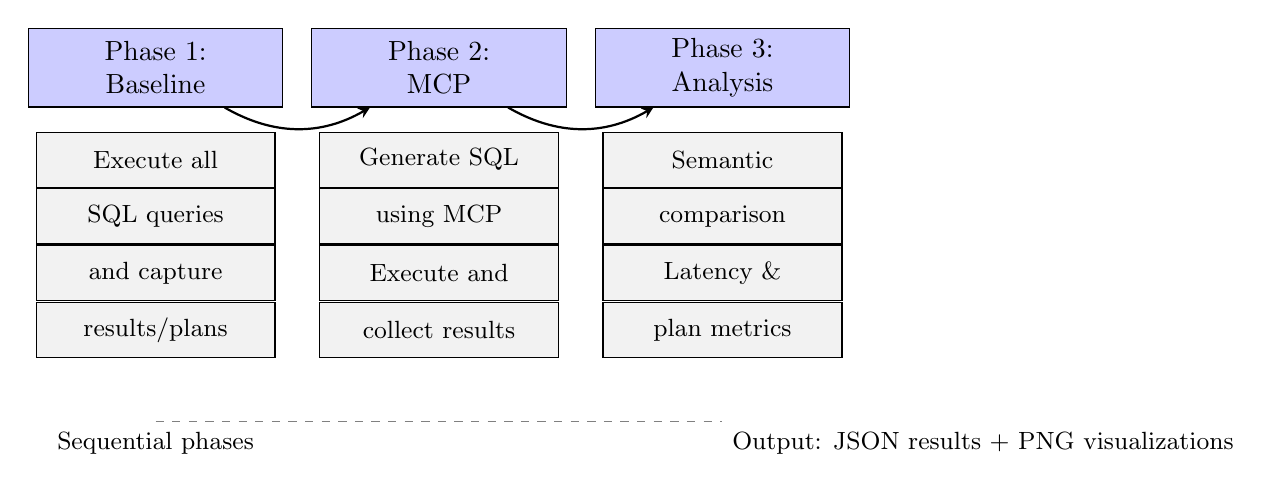
\begin{tikzpicture}[scale=0.9]
  \tikzstyle{phase} = [rectangle, draw, fill=blue!20, text width=3cm, text centered, minimum height=1cm]
  \tikzstyle{arrow} = [thick,->,>=stealth]
  \tikzstyle{detail} = [rectangle, draw, fill=gray!10, text width=2.8cm, text centered, font=\small, minimum height=0.7cm]

  % Phase 1
  \node [phase] (p1) at (0,3) {Phase 1:\\Baseline};
  \node [detail] (p1d1) at (0,1.7) {Execute all};
  \node [detail] (p1d2) at (0,0.9) {SQL queries};
  \node [detail] (p1d3) at (0,0.1) {and capture};
  \node [detail] (p1d4) at (0,-0.7) {results/plans};

  % Phase 2
  \node [phase] (p2) at (4,3) {Phase 2:\\MCP};
  \node [detail] (p2d1) at (4,1.7) {Generate SQL};
  \node [detail] (p2d2) at (4,0.9) {using MCP};
  \node [detail] (p2d3) at (4,0.1) {Execute and};
  \node [detail] (p2d4) at (4,-0.7) {collect results};

  % Phase 3
  \node [phase] (p3) at (8,3) {Phase 3:\\Analysis};
  \node [detail] (p3d1) at (8,1.7) {Semantic};
  \node [detail] (p3d2) at (8,0.9) {comparison};
  \node [detail] (p3d3) at (8,0.1) {Latency \&};
  \node [detail] (p3d4) at (8,-0.7) {plan metrics};

  % Phase arrows
  \draw [arrow] (p1) to[bend right] (p2);
  \draw [arrow] (p2) to[bend right] (p3);

  % Detail arrows
  \draw [arrow, draw=none] (p1) -- (p1d1);
  \draw [arrow, draw=none] (p2) -- (p2d1);
  \draw [arrow, draw=none] (p3) -- (p3d1);

  % Timeline annotation
  \draw [gray, dashed] (0,-2) -- (8,-2);
  \node at (0,-2.3) [font=\small] {Sequential phases};
  \node at (8,-2.3) [font=\small, right] {Output: JSON results + PNG visualizations};
\end{tikzpicture}
\caption{Three-Phase Evaluation Protocol. (1) Baseline phase executes all gold-standard SQL queries and captures row results, execution plans, and latency. (2) MCP phase generates SQL from natural language using Claude API over REST, executes generated queries, and measures MCP latency overhead. (3) Analysis phase performs semantic comparison via normalized tuple sorting and extracts query optimization metrics from EXPLAIN PLAN output.}
\label{fig:evaluation_protocol}
\end{figure}
